% Admissibility and informedness: where a candidate heuristic may lie.
\documentclass[tikz,border=0pt]{standalone}
\usepackage{tikz}
\usetikzlibrary{backgrounds,arrows.meta}
\definecolor{hdblue}{HTML}{1B4F8A}
\definecolor{hdred}{HTML}{A62B1F}
\begin{document}
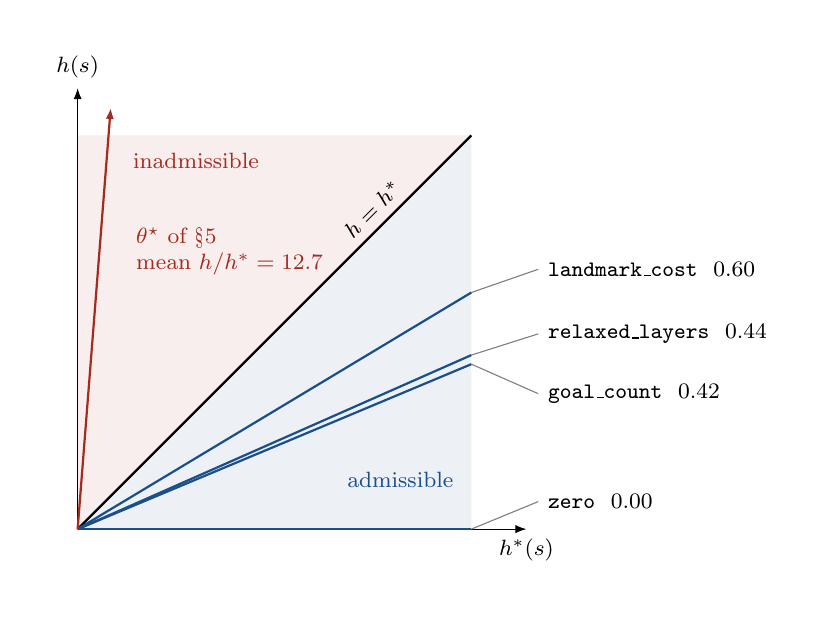
\begin{tikzpicture}[
    show background rectangle, inner frame sep=7pt,
    background rectangle/.style={fill=white},
    font=\footnotesize, >={Latex[length=4pt]}, x=1cm, y=1cm]

  % regions
  \fill[hdred!8]  (0,0) -- (5,5) -- (0,5) -- cycle;
  \fill[hdblue!8] (0,0) -- (5,5) -- (5,0) -- cycle;

  % axes
  \draw[->,black] (0,0) -- (5.7,0) node[anchor=north,pos=1] {$h^{*}(s)$};
  \draw[->,black] (0,0) -- (0,5.6) node[anchor=south,pos=1] {$h(s)$};

  % the boundary h = h*
  \draw[black,thick] (0,0) -- (5,5);
  \node[rotate=45,anchor=south west] at (3.5,3.5) {$h = h^{*}$};

  \node[hdred,  anchor=north west] at (0.58,4.90) {inadmissible};
  \node[hdblue, anchor=north west] at (3.30,0.85) {admissible};

  % mean rays; the gradient of each is that heuristic's mean h / h*
  \draw[hdblue,thick] (0,0) -- (5,3.005);
  \draw[hdblue,thick] (0,0) -- (5,2.210);
  \draw[hdblue,thick] (0,0) -- (5,2.095);
  \draw[hdblue,thick] (0,0) -- (5,0);

  % leaders and labels
  \draw[gray,thin] (5,3.005) -- (5.85,3.30);
  \draw[gray,thin] (5,2.210) -- (5.85,2.48);
  \draw[gray,thin] (5,2.095) -- (5.85,1.72);
  \draw[gray,thin] (5,0.000) -- (5.85,0.35);
  \node[anchor=west] at (5.85,3.30) {\texttt{landmark\_cost} \ 0.60};
  \node[anchor=west] at (5.85,2.48) {\texttt{relaxed\_layers} \ 0.44};
  \node[anchor=west] at (5.85,1.72) {\texttt{goal\_count} \ 0.42};
  \node[anchor=west] at (5.85,0.35) {\texttt{zero} \ 0.00};

  % the inadmissible candidate of section 5
  \draw[hdred,thick,->] (0,0) -- (0.42,5.35);
  \node[hdred,anchor=north west,align=left] at (0.62,3.95)
       {$\theta^{\star}$ of \S5\\ mean $h/h^{*} = 12.7$};
\end{tikzpicture}
\end{document}
